\documentclass[a4paper]{report}
\usepackage[utf8]{inputenc}
\usepackage{graphicx} % Required for inserting images
\usepackage{amsmath}
\usepackage{amssymb}
\usepackage{bookmark}
\usepackage{titlesec}
% \usepackage[T1]{fontenc}
% \usepackage{pgfplots} 
% \usepackage[myheadings]{fullpage}
% \usepackage{tikz}
\usepackage{hyperref}
% \usepackage{float}
\usepackage{fancyhdr}
% \usepackage{enumitem}
% \usepackage{changepage}
% \usepackage{subcaption} % loads the caption package
\usepackage{import}
\usepackage{geometry}
\usepackage[style=vancouver]{biblatex}

\addbibresource{all.bib}

\setlength{\parindent}{0px}
\pagestyle{fancy}

\geometry{
  a4paper,
  total={170mm,257mm},
  left=25mm,
  right=25mm,
  top=20mm,
}

% Header and footer information
\fancyhf{}
\setlength\headheight{15pt}
\fancyhead[L]{\thetitle} 
\fancyhead[R]{}
\fancyfoot[R]{\thepage}

\newcommand{\HRule}[1]{\rule{\linewidth}{#1}}

\titleformat{\chapter}[display]
  {\bfseries\Large}
  {}
  {0ex}
  {\titlerule\vspace{1ex}\filleft}
  [\vspace{1ex}\titlerule]

\title{Optimizing switch states in distribution grids}
\author{Sidney Pauly}
\date{March 2024}

% \graphicspath{img/ABDN.png}
\begin{document}

\begin{titlepage}
	
	\begin{center}
		
\includegraphics[width=50mm]{img/ABDN.png}\\[.5cm]
		School of Natural and Computing Sciences\\
		\HRule{2pt} \\
		\LARGE \textbf{Optimizing switch states in distribution grids}
		\HRule{2pt} \\ [0.5cm]
	\end{center}


\end{titlepage}

% \title{ UNIVERSITY OF ABERDEEN
% 		\\ [1.0cm]
% 		% Change to your faculty if needed
% 		
\includegraphics[width=50mm]{img/ABDN.png}\\[.5cm]
% 		School of Natural and Computing Sciences\\
% 		\HRule{2pt} \\
% 		\LARGE \textbf{Optimizing switch states in distribution grids}
% 		\HRule{2pt} \\ [0.5cm]
% 		\normalsize \today\vspace*{5\baselineskip}}
		
\tableofcontents

\chapter{Introduction}

% \section{Introduction}

The electrical grid is divided into multiple levels. Whilst the higher levels of the grid connect
the entire countries the lower level grids go from house to house and are hence also called 
distribution grids. In the past electricity was mostly produced at higher levels in power plants
and consumed at the lower level. The load patterns in the lower levels of the grid where
mostly predictable as they closely followed peoples work days. All this meant that a simpler setup
in the these girds was sufficient. In the past 20-30 this has changed. A lot of energy is now
being produced at these lower levels, e.g. through solar panels. Further, load patterns have shifted
as well with people charging their electric cars, heating with heat pumps and generally consuming
their energy at different times (e.g. because of home office)\autocite{venios}.
To fix load and instability issues arising
from this, there are broadly two options, either you build more physical infrastructure "blindly" to always
have a safe margin or you gather insight into the grid by measuring and simulating laods. This can either
be used in real time to actively control the grid or beforehand to have a better idea of load margins as well
as to more efficiently add new physical infrastructure. One active control measure that can be taken
to optimize load is by switching switches in the grid controlling how much of it is interconnected.
Generally a distribution grid connects up a few houses to a few streets depending on the region or country.
Each of these "grid islands" is connected up to the higher level through a transformer. By changing over
switches in the grid one can connect up these islands, making bigger grid areas or regroup certain parts
of these islands into neighbouring ones. Both can have effects on the grid in a non-linear complex way.\\



\chapter{Theory}

% \import{sections/theory/}{ac-basics.tex}

\section{AC Basics}

To the grid operates on alternating current, thus an
understanding of the underlying formulas governing ac systems will be required to analyse it. \\
In an AC system both current and voltage oscillate. This can be generally described using the following two equations:

\begin{equation}
    V(t) = V_m cos(\omega t + \theta_V)
    \label{eq:ac:voltage_ac}
\end{equation}

\begin{equation}
    I(t) = I_m cos(\omega t + \theta_I)
    \label{eq:ac:current_ac}
\end{equation}

where $V_m$ and $V_m$ are the magnitudes of voltage and current,
$\omega$ the angular velocity of the oscillations and $\theta_V$ and $\theta_I$
the phase offset of Voltage and current.\\
Power as a function of time can then be defined as:

\begin{equation}
    P(t) = V(t)I(t)
    \label{eq:ac:power_t}
\end{equation}

Expanding this leads to the following expression:

\begin{equation}
    \begin{aligned}
        P(t) = \frac{1}{2} V_m I_m (\cos (\theta_V-\theta_I) 
        + \cos(2(\omega t + \theta_V))\cos(\theta_V-\theta_I)
        + \sin(2(\omega t + \theta_V))\sin(\theta_V-\theta_I))
    \end{aligned}
    \label{eq:ac:power_ac_long}
\end{equation}

which can be simplified using

\begin{equation}
    \begin{aligned}
        &\text{Impedance angle}: \quad  \theta &= \theta_V - \theta_I \\
        &\text{Root mean square of } V: \quad  |V| &= \frac{V_m}{\sqrt{2}} \\
        &\text{Root mean square of } I: \quad  |i| &= \frac{I_m}{\sqrt{2}} \\
    \end{aligned}
    \label{eq:ac:power_def}
\end{equation}
         
\begin{equation}
    \begin{aligned}
        P(t)   &= P_R(t) + P_X(t)\\
        P_R(t) &= |V||I| \cos(\theta) (1 + \cos(2(\omega t+\theta_V)))\\
        P_X(t) &= |V||I| \sin(\theta) (1 + \sin(2(\omega t+\theta_V)))\\
    \end{aligned}
    \label{eq:ac:power_react_and_capacitive}
\end{equation}

If we are interested in steady state scenarios, then we can assume $\omega$ and $\theta_V$ 
to be constants. Over longer periods of time the average of $\sin(A t + B)$ and $\cos(A t + B)$ are 0.\\
We can thus simplify $P_R$ and $P_X$ further:

\begin{equation}
    \begin{aligned}
        P_R(t) &= P = |V||I| \cos(\theta)\\
        P_X(t) &= Q = |V||I| \sin(\theta)\\
    \end{aligned}
    \label{eq:ac:power_react_and_imag}
\end{equation}

It is handy to define these as the real and imaginary parts of a complex number:

\begin{equation}
    \begin{aligned}
        S     &=  V I^*\\
        S     &= P - iQ\\
        Re(S) &= P\\ 
        Im(S) &= Q
    \end{aligned}
    \label{eq:ac:complex}
\end{equation}

To describe an AC grid we also need to introduce a complex version
of Ohm's law:

\begin{equation}
    V = ZI
    \label{eq:ac:ohm_complex}
\end{equation}

where $Z$ is impedance which is defined as:

\begin{equation}
    Z = R + iX
    \label{eq:ac:impedance}
\end{equation}

where $R$ is resistance and $X$ is reactance. Reactance measures how much
energy will be stored in the cable within a current cycle due to a magnetic
field being created\\

Lastly we can also define an ac-equivalent for conductance, which is called admittance $Y$:

\begin{equation}
    Y = 1/Z
    \label{eq:ac:admittance}
\end{equation}

\section{Powerflow}

To simulate the grid a way to solve the powerflow problem is needed. To solve powerflow we assume,
that we know all the production and consumption of all prosumers, as well as the voltage at the so-called slack
node (for this node the consumed/produced power is not known). Using a powerflow solver we can then determine the voltage
at all the other nodes in the grid as well as the power at the slack node. This information then also suffices to determine
the currents through all cables. Taken together these quantities give a fairly good overview over how the grid performs.

\begin{center}
    \begin{tabular}{ c c c c }
    Node type          & Power     & Voltage & Count \\ 
    \hline
    \textbf{Slack}     & Unknown   & Known   & 1     \\  
    \textbf{Prosumer}  & Known     & Unknown & n    
    \end{tabular}
\end{center}



To formulate the powerflow equation, we can start form the general assumption
that the current entering node has to equal the current exiting it.\\
There is two sources for current through a node:

\begin{itemize}
    \item Current due to the prosumer at that node
    \item Current from or to other nodes
\end{itemize}

Defining the current due to the node itself is straight forward by considering
the complex power equation (eq: \ref{eq:ac:complex}):

\begin{equation}
    \begin{aligned}
        S_i     &= V_iI_i^*\\
        I_i     &= \frac{S_i^*}{V_i^*}
    \end{aligned}
    \label{eq:pf:current_due_to_prosumer}
\end{equation}

Defining the current due to the other nodes requires the use of Ohm's law (eq. \ref{eq:ac:ohm_complex}).
The current flowing from the current node (node $i$)
to one of the adjacent nodes (node $j$) will be a result of the
voltage difference between the current node and its neighbour:

\begin{equation}
    \begin{aligned}
        \Delta V_{ij} &= Z_{ij} I_{ij} \\
        I_{ij}        &= (V_i - V_j) y_{ij}
    \end{aligned}
\end{equation}

Where $y_ij$ is the admittance between nodes $i$ and $j$.
Summing up all currents from all the neighbours (we can ignore the case $i = j$ as $\Delta V_{ii} = 0$)

\begin{equation}
    \begin{aligned}
        I_{i} &= \sum_{i \ne j}^N (V_i - V_j) y_{ij}\\
              &= V_i \sum_{i \ne j}^N y_{ij} - \sum_{i \ne j}^N V_j y_{ij}
        \label{eq:pf:current_at_node}
    \end{aligned}
\end{equation}

Finally, equating the two sources for current we get to the formulation of the power flow
equation:

\begin{equation}
    \begin{aligned}
        V_i \sum_{i \ne j}^N y_{ij} - \sum_{i \ne j}^N V_j y_{ij} = \frac{S_i^*}{V_i^*}
        \label{eq:pf:pf_eq_large}
    \end{aligned}
\end{equation}

One further simplification can be employed by using an admittance matrix, in it the diagonal elements are populated with the
so called self-admittance. It consists of the sum of admittances to the neighbouring nodes:

\begin{equation}
    y_{ii} = \sum_{i \ne j} y_{ij}
\end{equation}

Thus equation \ref{eq:pf:pf_eq_large} can be further simplified:

\begin{equation}
    \sum_{j=1}^N V_j y_{ij} = \frac{S_i^*}{V_i^*}
    \label{eq:pf:full_pf_eq}
\end{equation}

This powerflow equation is non-linear, which thus necessities the use of a computational
solver. Two solvers, their advantages and disadvantages as well as implementation details will
be discussed subsequently.\\


\section{Graph theory}

The electrical grid can be represented as a graph. 
In a graph theory a graph is defined as a set of nodes and edges. A node
is some point in the graph, whilst an edge is a connecting element between exactly
two nodes.\\
\\

The simplest form of a graph is where the nods and edges do not have
any additional information attached to them and the edges are bidirectional.
I.e. the edge $A \to B$ is the same as the edge $B \to A$. Even though the setup
of such a graph seems simple, there are numerous metrics and complicated questions
that can be asked at this level. For example trying to find the quickest way between
two points in a graph is already a non-trivial problem that has its own class of algorithms
(e.g. A*, etc.). In the context of this project graph-theory becomes important in two ways.
Firstly it informs how the grid data is represented and processed and secondly it can
be used to classify certain configurations of the grid, through graph measures.

\subsection{Grid data representation}

In the most fundamental terms the grid can be represented as nodes, which are the 
producers or consumers (also called prosumers) and cables, which are the edges.
The prosumers have a production or consumption capacity $S_i$ (complex power see eq. \ref{eq:ac:complex}).
The cables have an admittance $Y_{ij}$ (see eq. \ref{eq:ac:admittance}).\\
\\
3 ways to represent the graph data will be subsequently used. 
Each records the full information of the graph, but
has different advantages and disadvantages. Note that the examples shown below all record
the admittance of each cable in addition to the info that the cable exists. Sometimes
this info is not need in which case it can be omitted and the representation further simplified/

\subsubsection{Edge list}

In edge list representation there is an entry for each edge in the graph in form of a vector:

\begin{equation}    
    \mathfrak{E_{ij}} = (i,\ j,\ Y_{ij})
\end{equation}

here $i$ and $j$ are the index of node A and B connected by the edge and
$Y_{ij}$ the admittance of the edge (cable).
For sparse graphs (graphs where only a handful of all possible edges $\mathfrak{E_{ij}}$ exist), this method
of storing the graph data is very efficient as only as many entries as cables are required. The disadvantage
algorithmically is that finding a specific connection between is not so efficient as it has to be searched for amongst
all entries. E.g. to look up admittance between nodes a and b that specific edge has to be found.

\subsubsection{Matrix form}

In matrix form each row and column represents a node. Each entry in the matrix is the admittance between nodes $i$ and $j$.
If the admittance is not to be recorded than if a node exists the entry can be set to 1 and if not to 0 instead:

\begin{equation}
    Y =
    \begin{pmatrix}
        Y_{11} & Y_{12} & ... & Y_{1n}\\
        Y_{21} & ...    & ... & ...   \\
        ...    & ...    & ... & ...   \\
        Y_{n1} & ...    & ... & Y_{nn}\\
    \end{pmatrix}
\end{equation}

As the cables in a grid are symmetrical (admittance is the same for current from a to b as it is form b to a), 
the matrix is symmetrical as well: $Y_{ij} = Y_{ji}$. Further in pure graph representation all diagonal elements are
zero as there are no cables running in a loop starting and ending at the same node.\\ 
One big advantage of this representation is that it allows for quick lookups, i.e. if one needs the admittance between nodes a and b
one can simply look up that entry in the matrix.\\
A closely related matrix is the admittance matrix, here the diagonal elements are populated with the
so called self-admittance, which consist of the sum of admittances to the neighbouring nodes:
\begin{equation}
    Y_{ii} = \sum_{i \ne j} Y_{ij}
\end{equation}

The admittance matrix is useful as it can be directly used in some mathematical
or physical formulas like Ohm's law:

\begin{equation}
    V = YI
\end{equation}

The disadvantage of this form of representation is that it is very space inefficient, as it requires
$N^2$ entries (where $N$ is the number of nodes). Especially for sparse graphs a lot of these entreis contain
zeros and are thus redundant. This drawback in memory and iteration efficiency
can be mitigated by clever data structure arrangement, which will be discussed later. 

\subsubsection{Node representation}

In the node representation the graph is represented by the connections
each node has and the admittance to each other node:

\begin{equation}
    \mathfrak{N_i} = \sum_{i \ne j, Y_{ij} > 0} (j, \ Y_{ij}) 
\end{equation}

This representation is especially useful for things like flooding algorithms where it is
relevant to know which nodes can be reached from any given node in question. 

\subsection{Graph measures}

\chapter{Methods}

\section{Data available through VEP}

The \textbf{V}enios\textbf{E}nergy\textbf{P}latform is a cloud application
developed and hosted by Venios. The customers are grid operators who can use
it to visualize the grid, track real time data, have it predict 
operational parameters such as prosumer loads and control the grid.
The long term aim of this project is to develop an algorithm that takes in
congested grid areas as its input and advises VEP on possible improved
switch states and their effects. This dissertation aims to implement the first step of this
process by taking in grid data from VEP and analysing it, trying to figure out
improved grid configurations. Data obtained for this project from VEP can broadly
be categorized
into topological and load profiles. Whilst the former is anything having to do with
the grid structure, its geographical location and its operating parameters the later
are production or consumption values over time for each of the prosumers.\\
All data is obtained over Venios' API, in json format. This means any
grid area of any VEP customer can be used for this analysis just by changing out
the request parameters and use of the relevant authorization tokens for that customer.
No code changes are required. This approach has the added advantage that any customer grid
data is only stored in memory and only temporarily on the machine running the analysis. This
has data privacy advantages.

\subsection{Topological grid data}

The grid data coming from VEP contains edges and nodes.
The subtypes with relevance to this work are listed in tables \ref{table:vep:nodes} and
\ref{table:vep:edges}\\
\\
\begin{figure}[H]
    \begin{tabular}{l p{3cm} p{8cm}}
        Name & Power production/consumption & Description\\
        \hline
        Domestic prosumer & Consumes power & A household consuming power. Power is mainly consumed in the morning and evenings when people are home\\
        Industry prosumer & Consumes power & A store or factory. Power is mainly consumed during work hours\\
        Solar panel       & Produces power & Produces power based on sunlight, thus most power produced in the summer at mid-day\\
        Other prosumers   & Produces and consumes power & Other prosumers, like electric car chargers, batteries, heat pumps, etc. These can have a range of load patterns\\
        Any other node    & None           & Any other node acting as a junction, busbar or other. As they all do not consumer or produce power they are only relevant as so far as they act as junctions for cable connections
    \end{tabular}
    \caption{Node types relevant to this work}
    \label{table:vep:nodes}
\end{figure}

\begin{figure}[H]
    \begin{tabular}{l p{10cm}}
        Name & Description\\
        \hline
        Cable & Cables have impedance and a physical length\\
        Transformer & Connects a grid to a higher voltage level. Main feed-in point in a low voltage grid\\
        Switch & An edge that can be interrupted. Modelled with no impedance and no physical length\\
        Any other & Other miscellaneous edge not modelled with physical length or impedance. Usually connects nodes within a substation or electrical cabinet.
      \end{tabular}
    \caption{Edge types relevant to this work}
    \label{table:vep:edges}
\end{figure}

A good dataset for validation and comparison is the SimBench data set. It is a set of
gird data provided by the University Kassel. The dataset aims to model typical German
grids in rural and urban environments. It was specifically designed to include a higher
number of renewables in the low voltage level, like solar panels\autocite{simbench}. These
simbench grids can be also imported in VEP and where thus used as the initial validation case
for this work.\\

Figure \ref{fig:vep:simbench_node_types} shows one of these Simbench grids ("1-LV-rural1"). 
Within VEP this grid is modelled with 553 edges and 553 nodes. A lot of these nodes are there to model
internals like bus bars or protective switch setups. For power flow and for analysing
switch states these nodes can be merged down to 96 with 95 edges running between them. 
The exact method to do so will be explained in the data preparation section. These numbers of nodes
are typical for German grids\autocite{venios}.

\begin{figure}[h]
    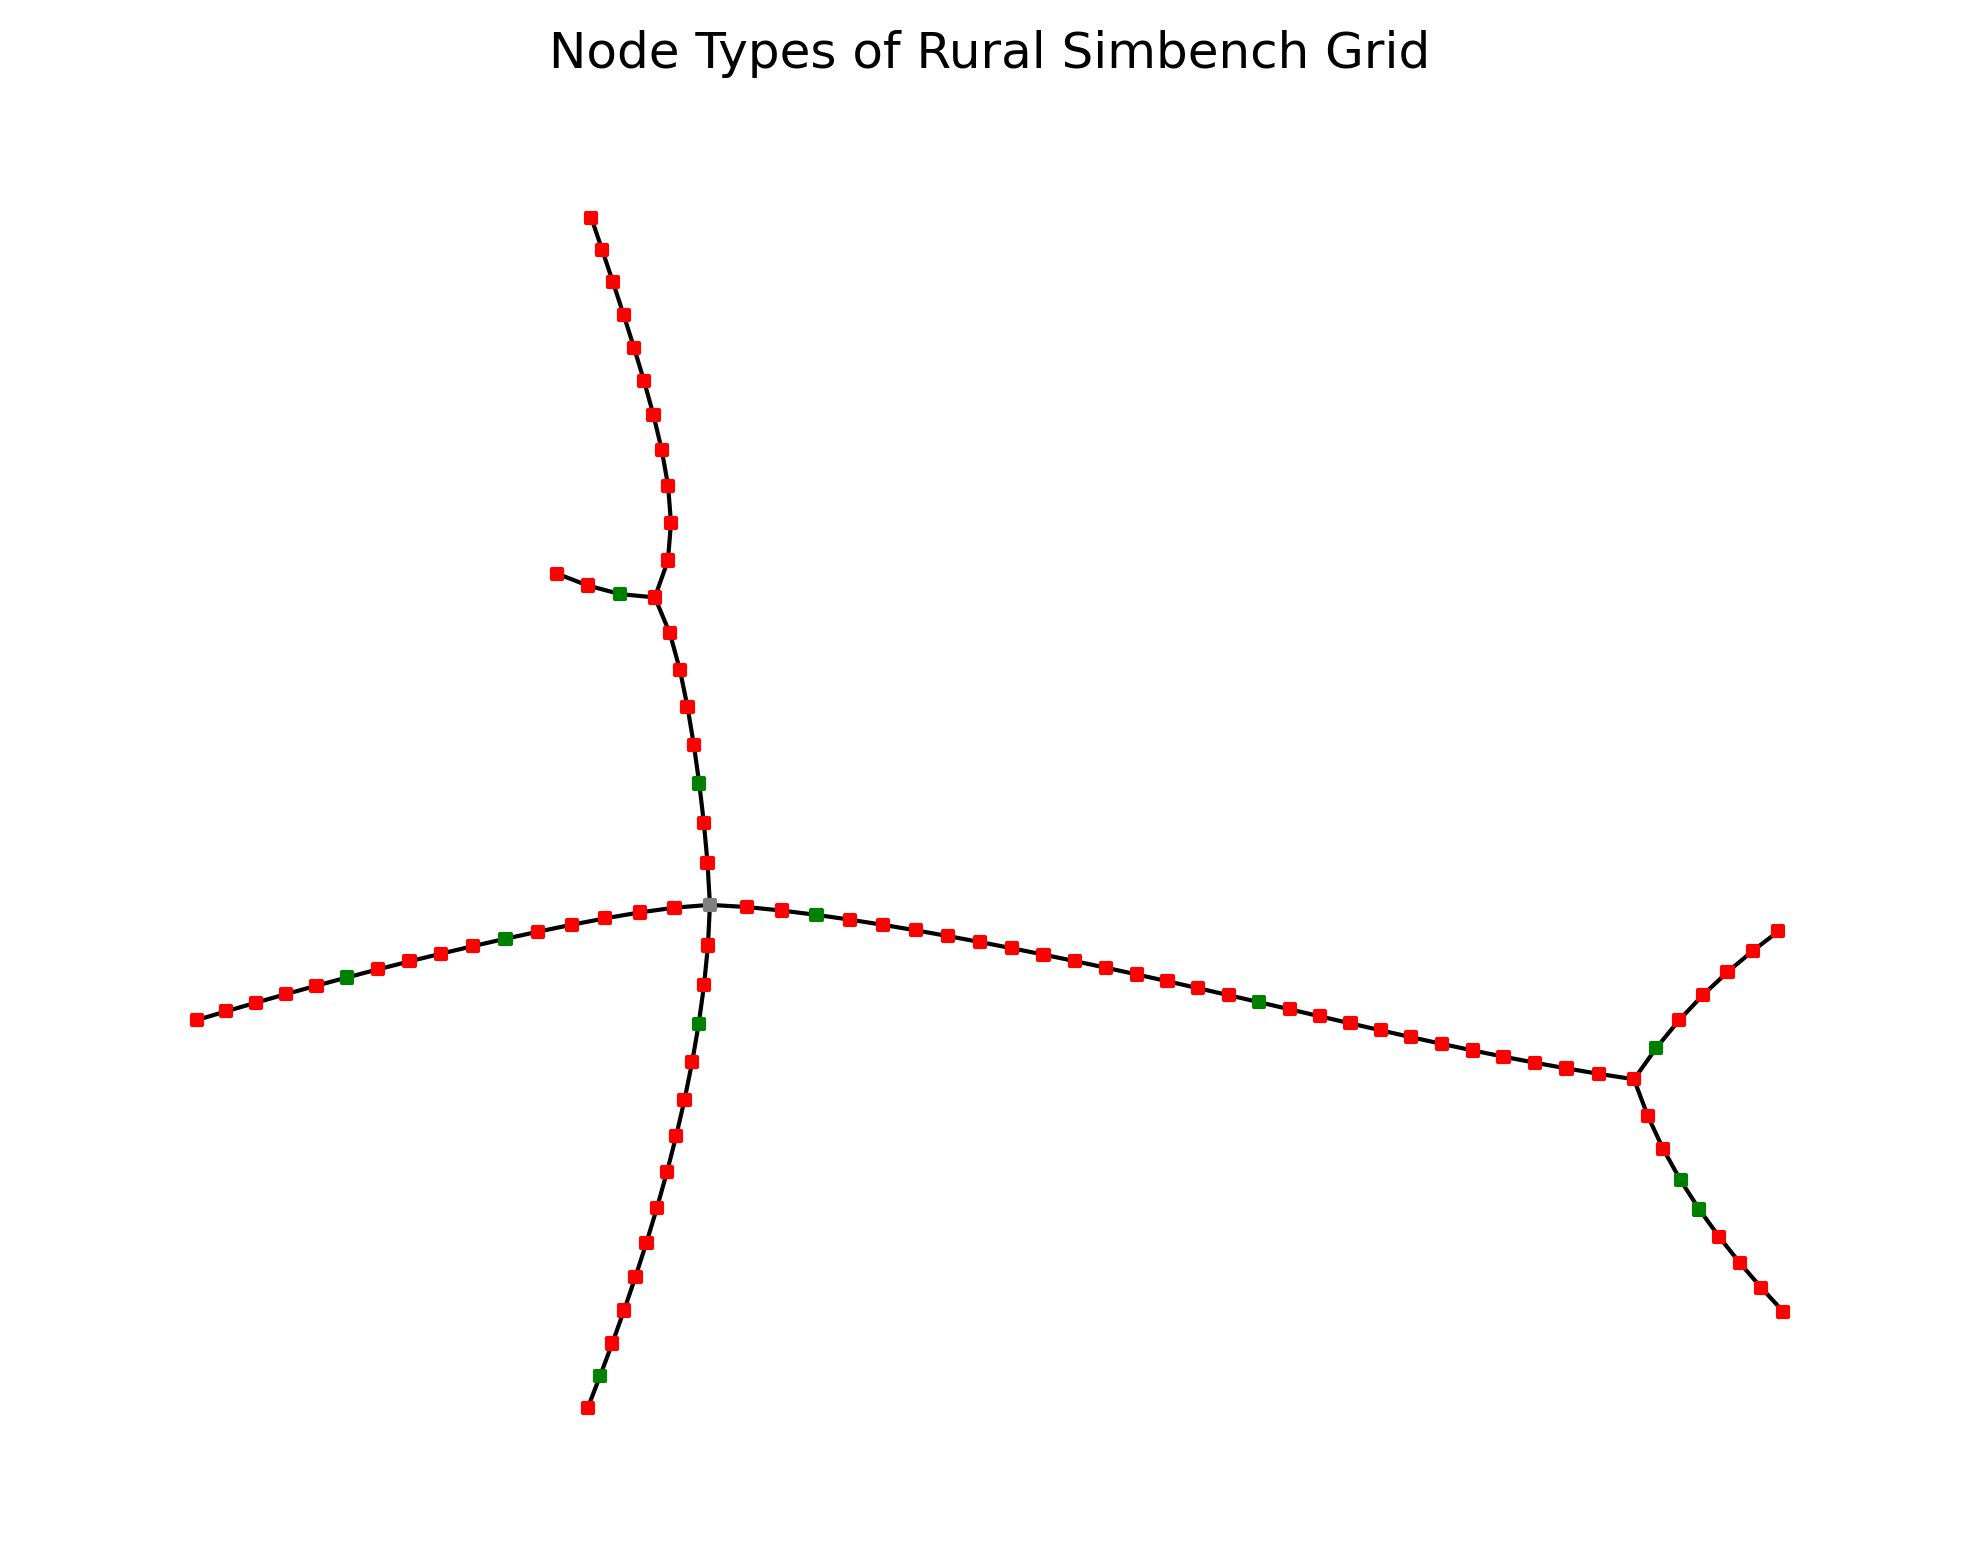
\includegraphics{img/simbench/layout.png}
    \caption{
        Non-geographical representation of the SimBench "1-LV-rural1"
        grid\autocite{simbench}. Layout produced with
        Kamada-Kawai layout algorithm\autocite{kamada_kawai}.
        Nodes with connected transformers are shown
        in \textbf{grey}, households with solar panels in \textbf{green}
        and normal households in \textbf{red}. Only cables with non-zero impedance shown, any nodes
        connected by zero impedance cables have been merged.
    }
    \label{fig:vep:simbench_node_types}
\end{figure}

% The grouping into grids
% Outer world (for geographical locations)
%   Nodes
%   Edges
% Inner world (conducting)
%   Nodes (simple, prosumer, slack)
%   Edges (switches, simple, with impedance, transformers)
% Standard switchstate

\subsection{Grid Load}

To simulate the grid adequately, production and consumption values for
each of the prosumers is needed. VEP provides various different models
to do so ranging form standard load profiles (standardized curves which are adjusted
according to the prosumer's parameters), neural network models trained on historic data,
weather forecast based models, and actual real time measurement values\autocite{venios}.\\
\\
Within real low voltage girds, the data available will often be spotty. Not all prosumers
have measurement devices and their measurement frequency is often limited. The most accurate
load modelling data is therefore often a mixture of the sources mentioned above.\\
\\ 
For this work all load time series will be obtained from Venios through its API. Venios works
closely with the grid operators to make sure these timelines most closely resemble the conditions
in the real grid. This important as these values are being used to monitor the grid and in some
cases trigger active control measures\autocite{venios}. Within this work it is assumed that the data
available through the API is the best data available, which closely resembles the actual grid load.
Any switch states and their effects on grid parameters will be tested against this data. It can
thus be reasonably assumed that any improvements seen based on this data translate reasonably well
into the real world. 

\begin{figure}[H]
    \begin{subfigure}{.5\textwidth}
      \centering
      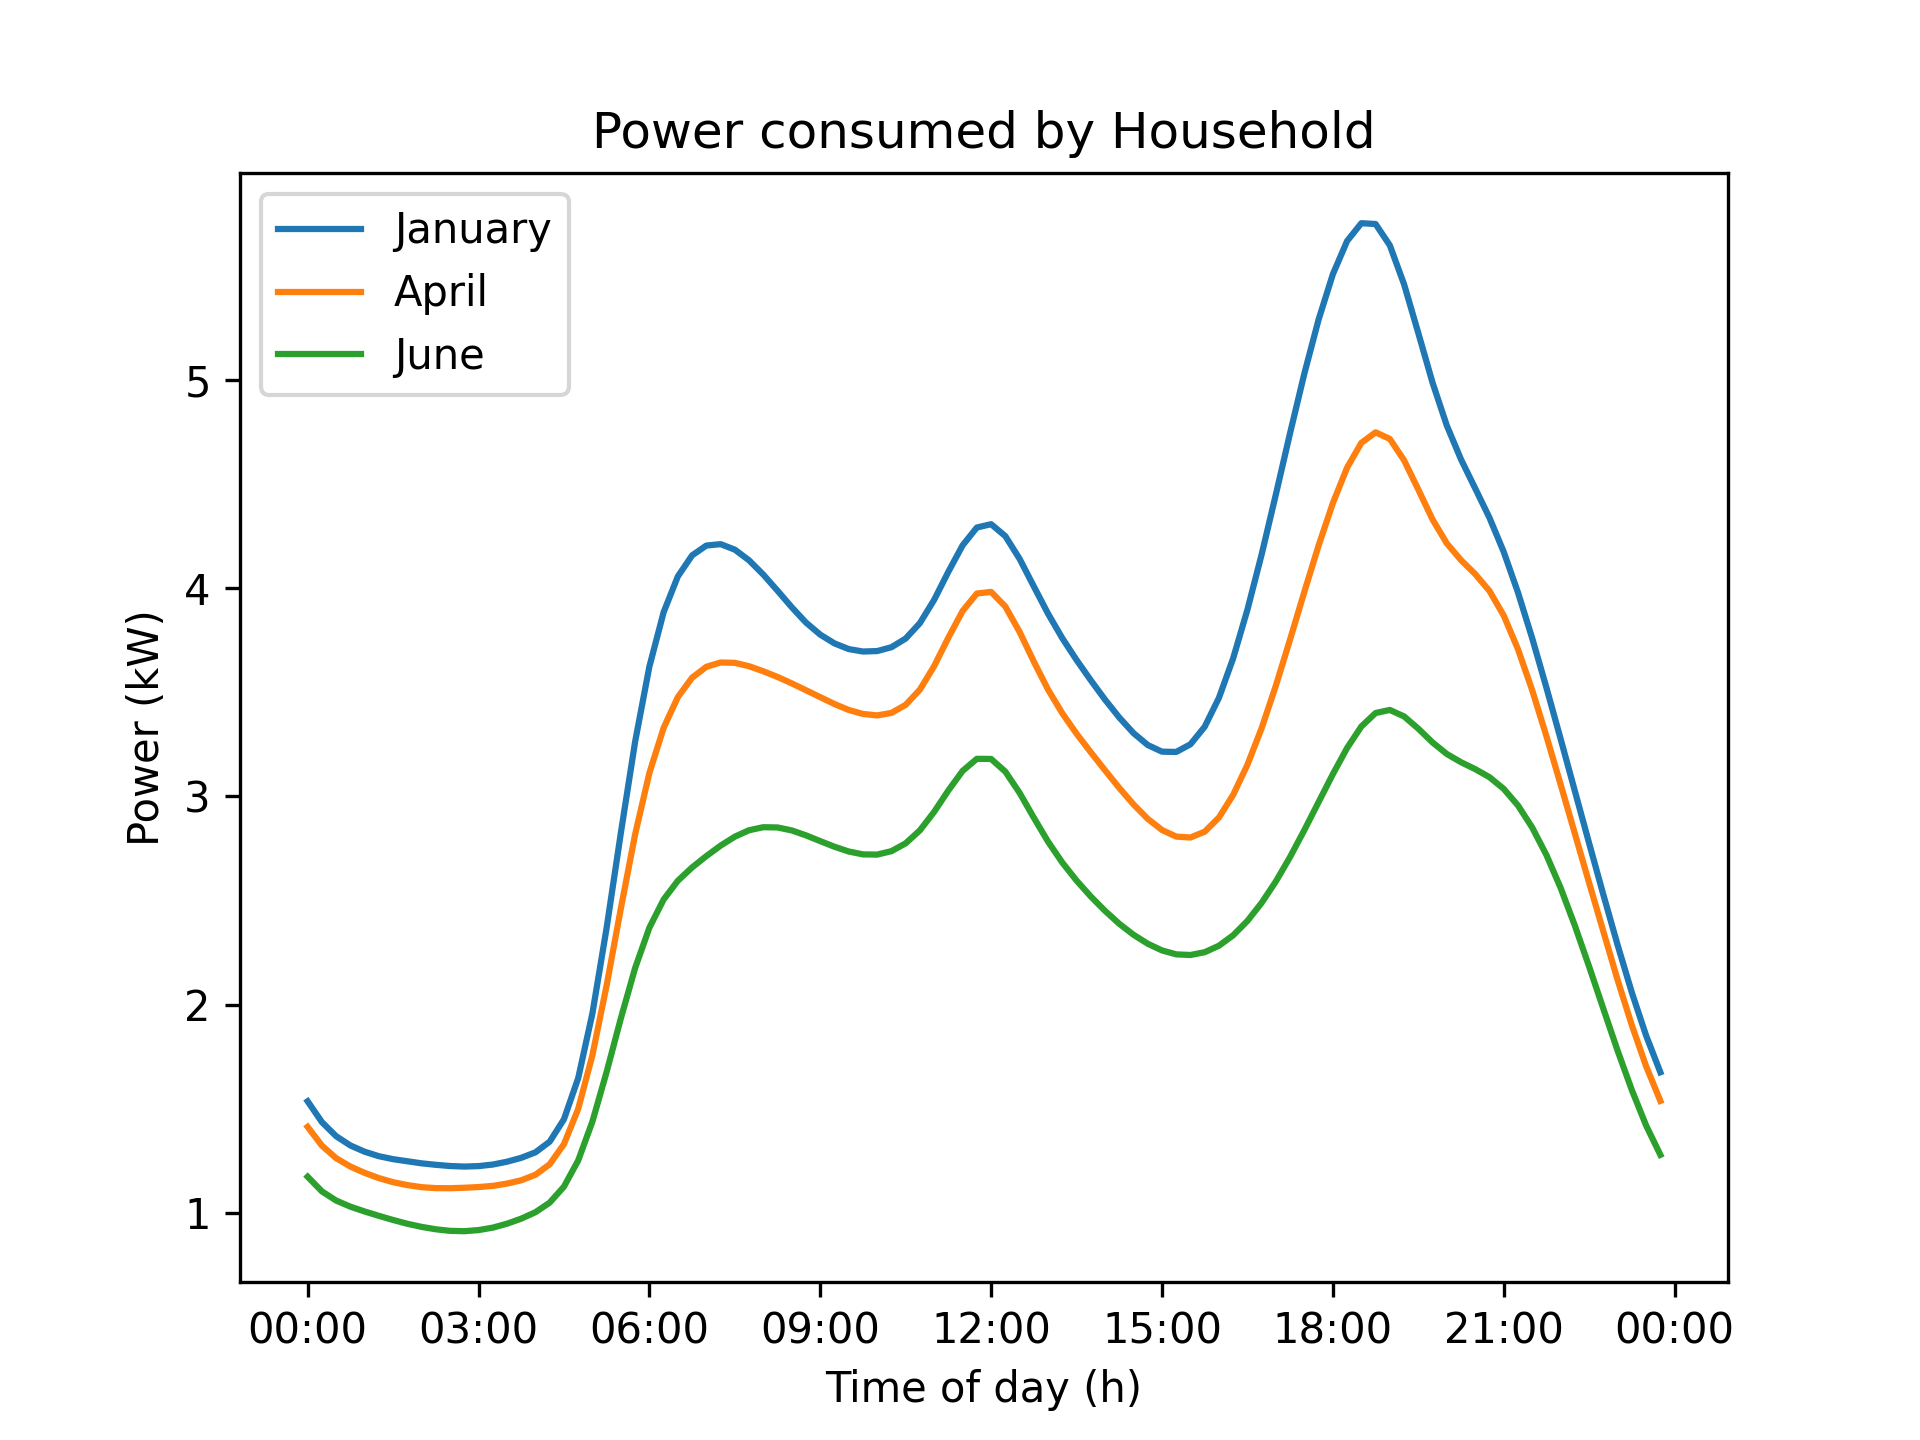
\includegraphics[width=\linewidth]{img/simbench/load_profile_household.png}
      \caption{}
      \label{fig:vep:load_profile_household}
    \end{subfigure}%
    \begin{subfigure}{.5\textwidth}
      \centering
      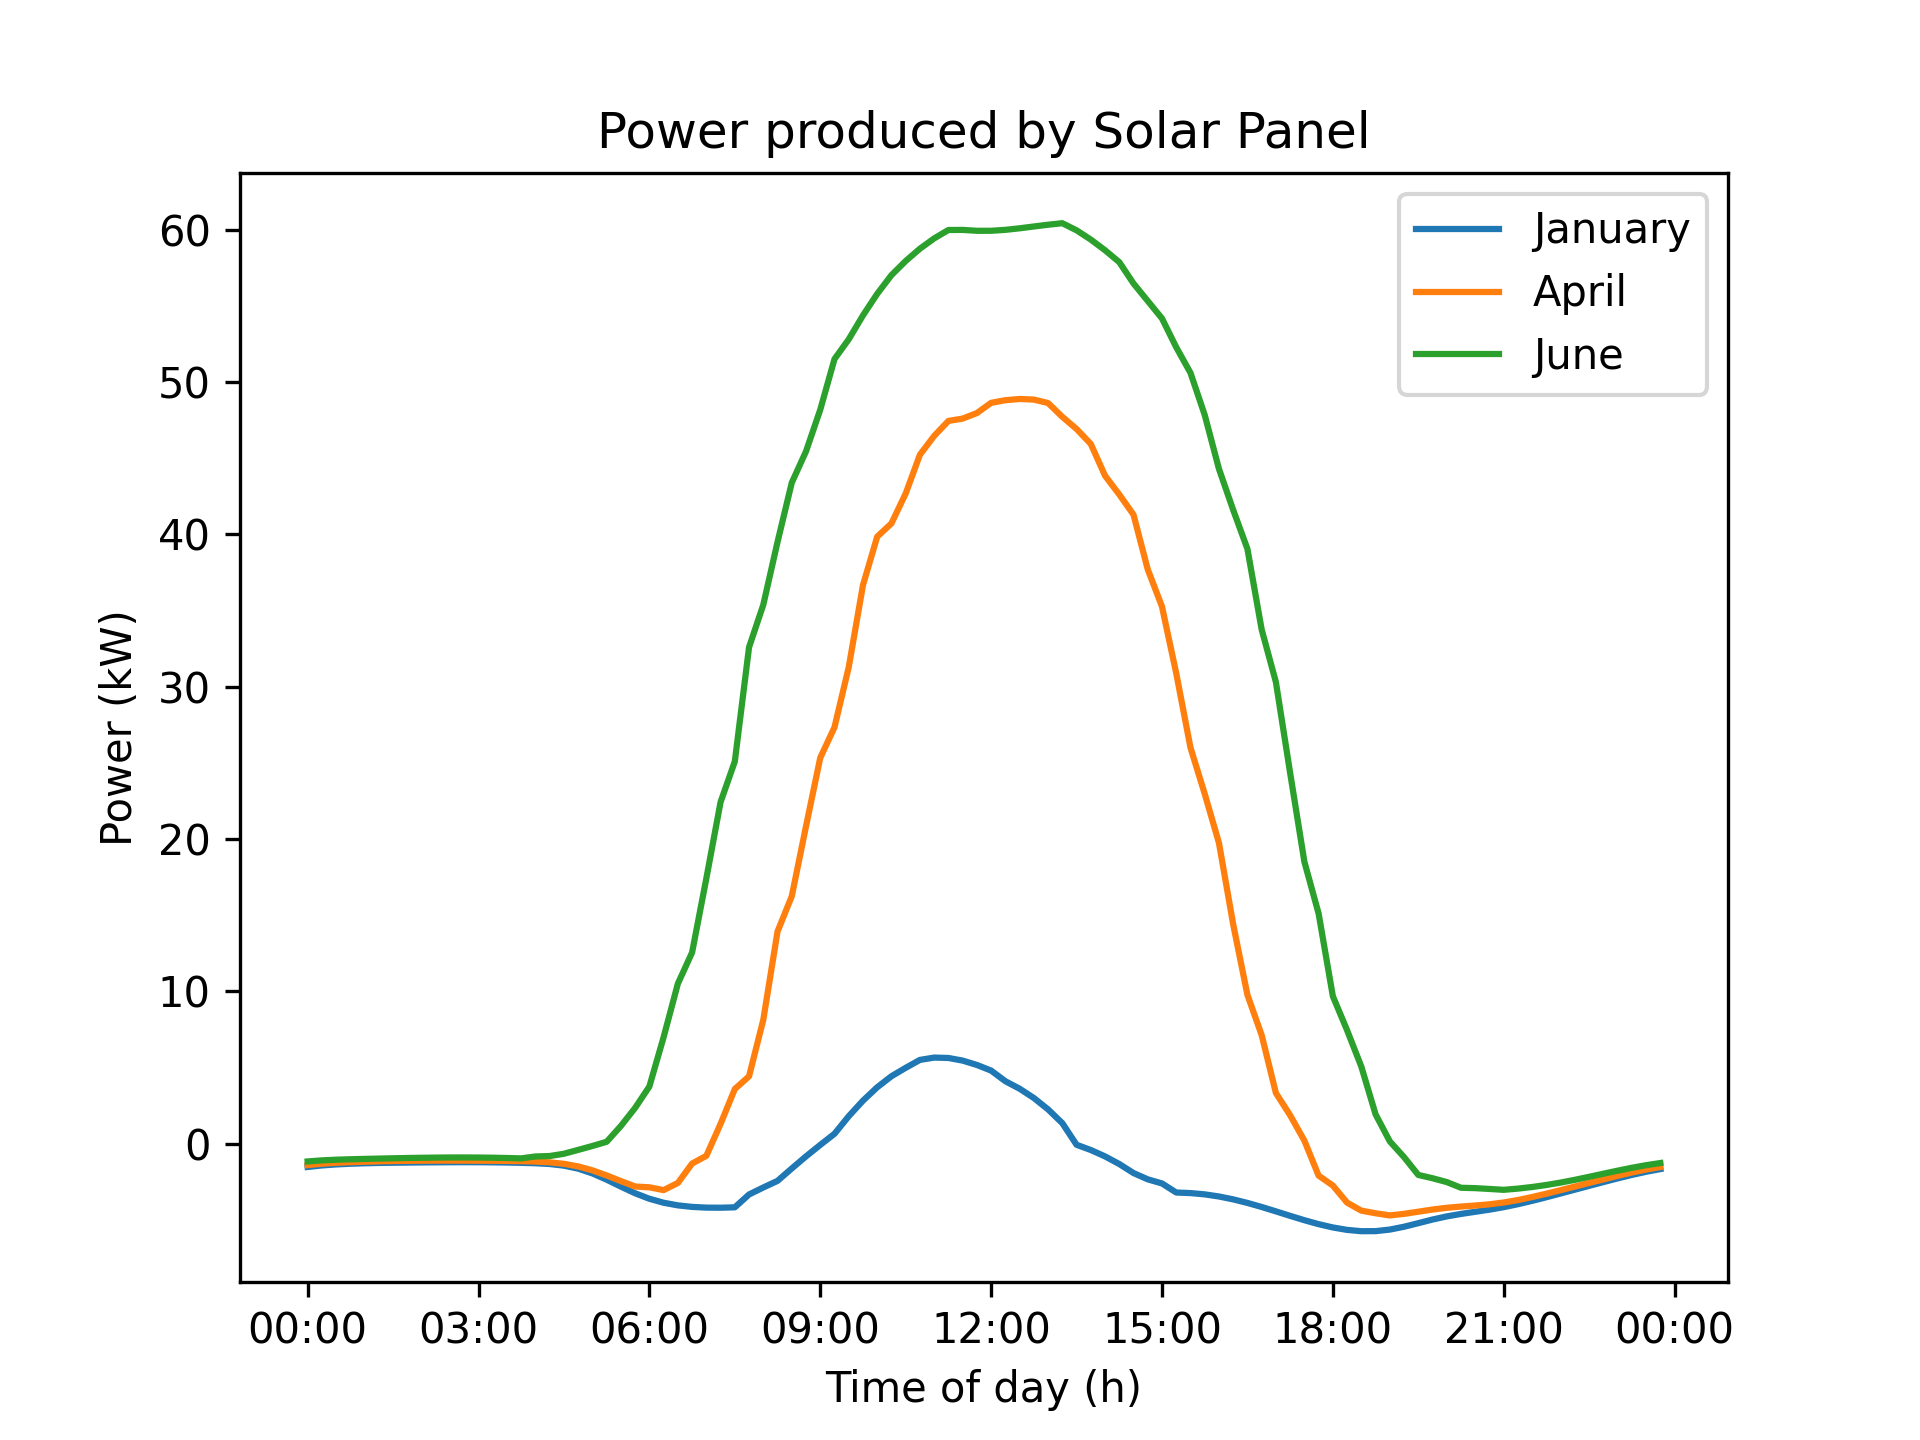
\includegraphics[width=\linewidth]{img/simbench/load_profile_solar.png}
      \caption{}
      \label{fig:vep:load_profile_solar}
    \end{subfigure}
    \caption{Power produced/consumed by a household (a) and a solar panel (b) within a SimBench grid at different times of day and at different times of year. Data is generated by a standard laod profile model within VEP and obtained over API\autocite{venios}}
    \label{fig:vep:load_profiles}
\end{figure}

Figure \ref{fig:vep:load_profiles} shows example load data obtained from VEP. It can be seen
that power production and consumption varies, widely throughout the day and the year. As a result the grid
might act very differently depending on the season and time. An important question to answer is therefore if
there are swtichstates that are generally better or if the best switch state is highly dependent on
time.\\
\\
Often switches within the grid can only be operated manually\autocite{venios}. Therefore, changing the grid configuration is linked to
some effort and cannot be done very often. If it turns out that there are switch states that are consistently better
a new and improved permanent switch state could be considered. If the best switch state is
however dependent on time, then depending on the scale of improvement, remotely controlled switches might be a worthwhile
investment.


\section{Data cleanup and preperation}

% Explain the atomic island concept
% Inter atomic-island switches
% Explain how this will be the grid we'll be optimizing on
% Explain that we can merge in the atomic islands acting as "leafs" (show comparison graph)grid
% Explain the problem with not connected parts of the grid in the satandard switch case and the solution

\section{Powerflow algorthms}

% Mention that the faster we can run powerflow the more data can be collected later -> a main goal
% is to make powerflow as fast as possible
% Validation:
%   1. Comparision with results obtained by book
%   2. Comparision with vep results?
% Gauss-Seidel
% Newton-raphson
% python-c adapter
% sparse matricies optimization
% Show performance of different methods over grid size?

\section{Switchstate explorer}

% Explain constraints: exactly one trafo per gird, no unconnected nodes 
% Metion literature: anchored graph partitioning

% Expalin algorithm:
% Explain random element

\section{Measures applied and justification}

% - power stats (avg, std, etc)
% - voltage stats
% - island size
% - atomic island count
% - line loading stats
% - trafo loading stats
% - net power (without trafo?)
% - geo extend stats
% - deveation from standard switchstate
% - networkx measures
% - Losses

\section{Scoring a switchstate}

% Explain simple method used

\chapter{Results}

\section{Proving the random switchstate generator works}

% Show distributions of pre-powerflow data (perhaps per grid)

\section{Happy case: suburban EWZ grid}

\section{Unhappy case: urban EWZ grid}

\section{Changing laod data over time}

\section{Wider sampling?}

\printbibliography

\end{document}